% vim: set foldmethod=marker foldlevel=0:

\documentclass[a4paper]{article}
\usepackage[UKenglish]{babel}

% NOTE: hyperref has to come before preamble
\usepackage{hyperref}

\usepackage{preamble}

\usepackage{graphicx}
\graphicspath{ {./imgs/} }

\fancyhead[L]{MA144 Assignment 3}
\title{MA144 Methods of Mathematical Modelling 2, Assignment 3}
\colorlet{questionbodycolor}{green!50}

\begin{document}

\maketitle

\setlength{\parindent}{0em}
\setlength{\parskip}{1em}

% {{{ Q1
\question{1}

\begin{questionbody}
Consider the volume of the solid $S$ bounded between the plane $z=1$ and the surface $z = x^2 + 4y^2$.
\end{questionbody}

\subsection{~} % 1.a

\begin{questionbody}
Express the volume as a triple integral in Cartesian coordinates. Do this in \textit{three} ways with different orders of integration.
\end{questionbody}

\begin{align*}
% S &= \intlim {}{} {\intlim {}{} {\intlim {}{} {} x} y} z\\[1ex]
S &= \intlim 01 {\intlim {-\f{\sqrt z}2}{\f{\sqrt z}2} {\intlim {-\sqrt{z - 4y^2}}{\sqrt{z - 4y^2}} {} x} y} z \\[2ex]
S &= \intlim 01 {\intlim {\sqrt z}{\sqrt z} {\intlim {-\sqrt{z - x^2}}{\sqrt{z - x^2}} {} y} x} z \\[2ex]
S &= \intlim {-\f12}{\f12} {\intlim {-\sqrt{1 - 4y^2}}{\sqrt{1 - 4y^2}} {\intlim {x^2 + 4y^2}{1} {} z} x} y
\end{align*}

\newpage
\subsection{~} % 1.b

\begin{questionbody}
Choose one of the triple integrals you wrote down in part \textbf{(a)}. Calculate the volume of the solid.
\end{questionbody}

\begin{align*}
S &= \intlim {-\f12}{\f12} {\intlim {-\sqrt{1 - 4y^2}}{\sqrt{1 - 4y^2}} {\intlim {x^2 + 4y^2}{1} {} z} x} y \\[1ex]
&= \intlim {-\f12}{\f12} {\intlim {-\sqrt{1 - 4y^2}}{\sqrt{1 - 4y^2}} {\l( 1 - x^2 - 4y^2 \r)} x} y \\[1ex]
&= \intlim {-\f12}{\f12} {\l[ x - \f13 x^3 - 4xy^2 \r]_{x = -\sqrt{1 - 4y^2}}^{\sqrt{1 - 4y^2}} } y \\[1ex]
&= \intlim {-\f12}{\f12} {\l( k - \f13 k (1 - 4y^2) - 4k y^2 - \l( -k + \f13 k (1 - 4y^2) + 4k y^2 \r) \r)} y \\
&\quad \text{(where } k = \sqrt{1 - 4y^2}\, \text{)} \\[1ex]
&= \intlim {-\f12}{\f12} {\sqrt{1 - 4y^2} \l( 1 - \f13 (1 - 4y^2) - 4 y^2 + 1 - \f13 (1 - 4y^2) - 4 y^2 \r)} y \\[1ex]
&= \intlim {-\f12}{\f12} {\sqrt{1 - 4y^2} \l( 2 - \f23 (1 - 4y^2) - 8 y^2 \r)} y \\[1ex]
&= \intlim {-\f12}{\f12} {\sqrt{1 - 4y^2} \l( \f43 + \f83 y^2 - \f{24}3 y^2 \r)} y \\[1ex]
&= \intlim {-\f12}{\f12} {\sqrt{1 - 4y^2} \l( \f43 - \f{16}3 y^2 \r)} y \\[1ex]
&= \f43 \intlim {-\f12}{\f12} {\sqrt{1 - 4y^2} \l(1 - 4y^2 \r)} y \\[1ex]
&= \f43 \intlim {-\f12}{\f12} {\l(1 - 4y^2 \r)^{\f32}} y
\end{align*}
I don't know how to continue, but \href{https://www.sagemath.org/}{SageMath} says this integral is $\df\pi4$.
% }}}

% {{{ Q2
\newquestion{2}

\begin{questionbody}
A thin metal plate has mass $M$ and uniform density $\rho$ (where density in this case equals mass per unit area). The boundary of the plate is the polar curve $r = 1 + \sin \theta$.
\end{questionbody}

\subsection{~} % 2.a

\begin{questionbody}
Show that $M = \df{3 \pi \rho}2$.
\end{questionbody}

$\ds M = \iint_\Omega \rho \d A$ where $\Omega$ is the region defined by the curve $r = 1 + \sin \theta$. Therefore \begin{align*}
M &= \intlim 0{2\pi} {\intlim 0 {1 + \sin \theta} {\rho r} r} \theta\\[1ex]
&= \f\rho2 \intlim 0{2\pi} {\l[ r^2 \r]_0^{1 + \sin \theta}} \theta\\[1ex]
&= \f\rho2 \intlim 0{2\pi} {\l( 1 + 2\sin\theta + \sin^2 \theta \r)} \theta\\[1ex]
&= \f\rho2 \intlim 0{2\pi} {\l( 1 + 2\sin\theta + \f12 - \f12 \cos 2\theta \r)} \theta\\[1ex]
&= \f\rho4 \intlim 0{2\pi} {\l( 3 + 4\sin\theta - \cos 2\theta \r)} \theta\\[1ex]
&= \f\rho4 \l[ 3\theta - 4\cos\theta - \f12 \sin 2\theta \r]_0^{2\pi}\\[1ex]
&= \f\rho4 \l( 6\pi - 4 + 0 - \l( 0 - 4 - 0 \r) \r)\\[1ex]
&= \f{6\pi \rho}4\\[1ex]
&= \f{3\pi \rho}2\\[1ex]
\end{align*}

\subsection{~} % 2.b

\begin{questionbody}
Locate the centre of mass $(\overline x, \overline y)$ of the plate.
\end{questionbody}

$\ds \overline x = \f1M \iint_\Omega x \rho \d A$ and $\ds \overline y = \f1M \iint_\Omega y \rho \d A$, where $x = r\cos\theta$ and $y = r\sin\theta$.

Therefore \begin{align*}
\overline x &= \f2{3\pi\rho} \intlim 0{2\pi} {\intlim 0 {1 + \sin \theta} {\rho r^2 \cos \theta} r} \theta \\[1ex]
&= \f2{9\pi} \intlim 0{2\pi} {\cos \theta \l[r^3\r]_0^{1 + \sin\theta}} \theta \\[1ex]
&= \f2{9\pi} \intlim 0{2\pi} {\cos \theta \l( 1 + 3\sin\theta + 3\sin^2 \theta + \sin^3 \theta \r)} \theta \\[1ex]
 &= \f2{9\pi} \intlim 0{2\pi} {\l( \cos\theta + 3\sin\theta \cos\theta + 3\sin^2 \theta \cos\theta + \sin^3 \theta \cos\theta \r)} \theta \\[1ex]
&= \f2{9\pi} \l[ \sin\theta + \f32 \sin^2 \theta + \sin^3 \theta + \f14 \sin^4 \theta\r]_0^{2\pi} \\[1ex]
&= \f2{9\pi} \times 0  \\[1ex]
&= 0
\end{align*}

And \begin{align*}
\overline y &= \f2{3\pi\rho} \intlim 0{2\pi} {\intlim 0 {1 + \sin \theta} {\rho r^2 \sin \theta} r} \theta \\[1ex]
&= \f2{9\pi} \intlim 0{2\pi} {\sin \theta \l[r^3\r]_0^{1 + \sin\theta}} \theta \\[1ex]
&= \f2{9\pi} \intlim 0{2\pi} {\sin \theta \l( 1 + 3\sin\theta + 3\sin^2 \theta + \sin^3 \theta \r)} \theta \\[1ex]
&= \f2{9\pi} \intlim 0{2\pi} {\l( \sin\theta + 3\sin^2 \theta + 3\sin^3 \theta + \sin^4 \theta \r)} \theta \\[1ex]
&= \f2{9\pi} \intlim 0{2\pi} {\l( \sin\theta + \f32 - \f32 \cos 2\theta + 3 \sin \theta \l(1 - \cos^2 \theta\r) + \l( \f12 - \f12 \cos 2\theta \r)^2 \r)} \theta \\[1ex]
&= \f2{9\pi} \intlim 0{2\pi} {\l( 4 \sin\theta + \f32 - \f32 \cos 2\theta - 3 \sin\theta \cos^2 \theta + \f14 - \f12 \cos 2\theta + \f14 \cos^2 2\theta \r)} \theta \\[1ex]
&= \f2{9\pi} \intlim 0{2\pi} {\l( 4 \sin\theta + \f74 - 2 \cos 2\theta - 3 \sin\theta \cos^2 \theta + \f14 \l( \f12 + \f12 \cos 4\theta \r) \r)} \theta \\[1ex]
&= \f2{9\pi} \intlim 0{2\pi} {\l( 4 \sin\theta + \f74 - 2 \cos 2\theta - 3 \sin\theta \cos^2 \theta + \f18 + \f18 \cos 4\theta \r)} \theta \\[1ex]
&= \f2{9\pi} \intlim 0{2\pi} {\l( 4 \sin\theta + \f{15}8 - 2 \cos 2\theta - 3 \sin\theta \cos^2 \theta + \f18 \cos 4\theta \r)} \theta \\[1ex]
&= \f2{9\pi} \l[ -4\cos\theta + \f{15}8 \theta - \sin^3 \theta + \f1{32}\sin 4\theta \r]_0^{2\pi} \\[1ex]
&= \f2{9\pi} \l( -4 + \f{15\pi}4 + 0 - \l( -4 + 0 \r) \r) \\[1ex]
&= \f2{9\pi} \, \f{15\pi}4 \\[1ex]
&= \f56
\end{align*}
% }}}

% {{{ Q3
\newquestion{3}

\subsection{~} % 3.a

\begin{questionbody}
The triple integral below represents the volume of a solid in $\R^3$. \[
\intlim 0{2\pi} {\intlim 0 1 {\intlim {r^2} {3-2r} r z} r} \theta .
\] Sketch the solid and evaluate the triple integral.
\end{questionbody}

\begin{figure}[h]
	\centering
	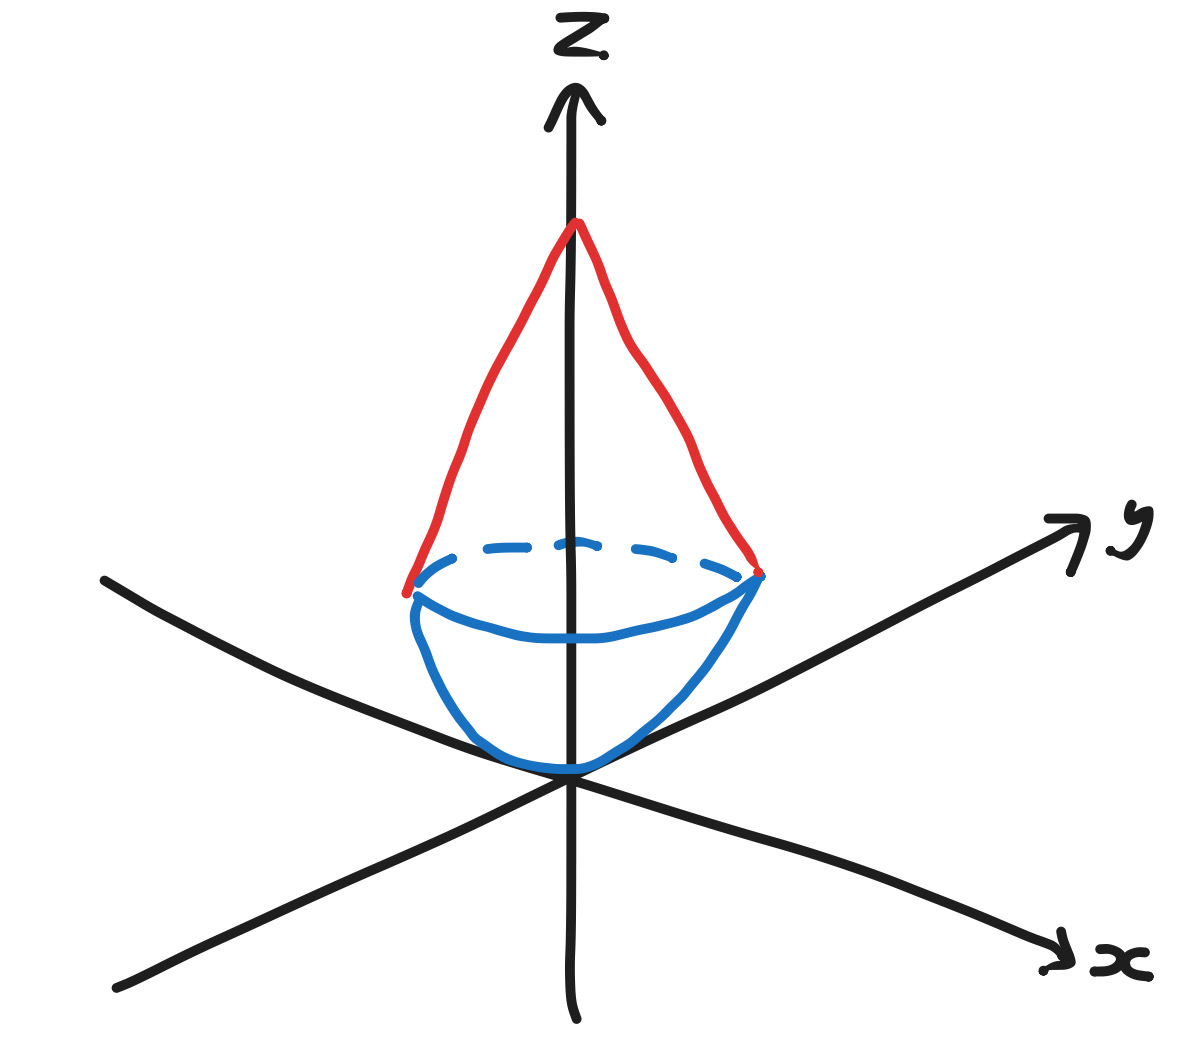
\includegraphics[scale=0.35]{Q3-sketch}
	\caption{A sketch of the solid}
\end{figure}

\begin{align*}
V &= \intlim 0{2\pi} {\intlim 01 {\intlim {r^2}{3-2r} r z} r} \theta\\[1ex]
&= \intlim 0{2\pi} {\intlim 01 {[rz]_{z=r^2}^{3-2r}} r} \theta\\[1ex]
&= \intlim 0{2\pi} {\intlim 01 {r \l( 3 - 2r - r^2 \r)} r} \theta\\[1ex]
&= \intlim 0{2\pi} {\intlim 01 {\l( 3r - 2r^2 - r^3 \r)} r} \theta\\[1ex]
&= \intlim 0{2\pi} {\l[ \f32 r^2 - \f23 r^3 - \f14 r^4 \r]_0^1} \theta
\end{align*}
\begin{align*}
&= \intlim 0{2\pi} {\l( \f32 - \f23 - \f14 \r)} \theta\\[1ex]
&= \intlim 0{2\pi} {\l( \f{18}{12} - \f8{12} - \f3{12} \r)} \theta\\[1ex]
&= \intlim 0{2\pi} {\f7{12}} \theta\\[1ex]
&= \f{7\pi}6
\end{align*}

\subsection{~} % 3.b

\begin{questionbody}
Evaluate the integral numerically using SciPy’s \texttt{tplquad} function. How accurate is Python’s answer? (i.e. to how many decimal places?)
\end{questionbody}

SciPy gives 3.6651914291880914 with an estimated error of approximately $4.07 \times 10^{-14}$. The actual answer is $\f{7\pi}6 = 3.665191429188092$, so SciPy is correct to 14 decimal places, which also matches the estimated error.

\begin{figure}[h]
	\centering
	\inputminted{python}{./code/Q3.py}
	\caption{The Python code used to generate this answer}
\end{figure}
% }}}

\end{document}
